% Metódy inžinierskej práce

\documentclass[10pt,twoside,slovak,a4paper]{article}

\usepackage[slovak]{babel}
%\usepackage[T1]{fontenc}
\usepackage[IL2]{fontenc} 
\usepackage[utf8]{inputenc}
\usepackage{graphicx}
\usepackage{url} 

%\usepackage{hyperref} 

\usepackage{cite}
%\usepackage{times}

\pagestyle{headings}

\title{Indexovanie veľkých dát v internete vecí: metódy a využitie\thanks{Semestrálny projekt v predmete Metódy inžinierskej práce, ak. rok 2023/24, vedenie: Pavol Baťalík}}

\author{Miloš Bardáč\\[2pt]
	{\small Slovenská technická univerzita v Bratislave}\\
	{\small Fakulta informatiky a informačných technológií}\\
	{\small \texttt{xbardac@stuba.sk}}
	}

\date{\small 30. september 2023}



\begin{document}

\maketitle

\begin{abstract}

V súčasnej dobe nepretržitého rastu objemu dát v oblasti internetu vecí je efektívne indexovanie neoddeliteľnou súčasťou. Z toho dôvodu sa tento článok zaoberá problematikou indexovania veľkých dát v IoT a rôznými technikami, ktoré sa využívajú v IoT prostredí. Okrem toho sa článok venuje aj požiadavkám a výzvam spojenými s indexovaním objemných dát v IoT. Medzi tieto výzvy patrí napríklad bezpezpečnosť a ochrana súkromia, cena, či postupom času veľký nárast objemu dát. Tento článok poskytuje pohľad na dôležitosť efektívneho indexovania v kontexte Internetu vecí a taktiež pomáha čitateľom lepšie pochopiť technikám indexovania a výzvam v tomto odvetví. Taktiež vysvetľuje prečo je rýchly a spoľahlivý prístup k dátam kľúčovým aspektom využitia IoT dát pre rôzne aplikácie a inovácie.

\end{abstract}


\section{Úvod}

Vstupujeme do doby, kedy sa svet okolo nás stáva čoraz viac prepojeným a inteligentným. Internet vecí, skrátene IoT, môžeme chápať ako súbor sietí, v ktorých sú fyzicky prepojené dáta alebo zariadenia, čo umožňuje týmto zariadeniam zhromažďovať a zdielať dáta. \cite{7916854} Práve táto technológia zohráva kľúčovú úlohu v tomto pomerne rýchlom pokroku. V poslednom čase môžme byť svedkami pomerne masivného nárastu objemu dát v oblasti internetu vecí. S týmto nárastom je spojená potreba tieto dáta efektívne usporiadávať a prehľadávať. 

Preto sa v následujúcich kapitolách bude článok venovať rôznym aspektom tohto nevyhnutného procesu. Hneď v následujúcej kapitole (časť ~\ref{poziadavky}) bude čitateľ oboznámený s požiadavkami spojenými s touto problematikou. Následujúca kapitola (časť ~\ref{oblasti}) je spojená so samotnými oblasťami využitia. V ďalšej časti (časť ~\ref{techniky}) sa článok zameriava na rôzne techniky indexovania objemných dát v oblasti Internetu vecí. Tie majú možnosť dosť výrazne zlepšiť rôzne odvetvia, či už je to priemysel, energetika či dokonca aj zdravotná starostlivosť. Jedná z posledných kapitol (časť ~\ref{vyzvy}) je venovaná problémom a výzvam, ktoré sa spájajú s touto tématikou. Patrí sem otázka bezpečnosti dát, ochrany súkromia používateľov, či správa zariadení. V predposlednej časti (časť ~\ref{zaver}) ukončíme tento článok záverom a zhrnutím. Zároveň v tejto časti si čitateľ pripomenie kľúčové body, ktorým sa článok venuje a taktiež sa dozvie o víziách tejto problematiky do budúcnosti. Na úplnom konci, posledná kapitola (časť ~\ref{temy}) bude obsahovať reakciu na témy z prednášok.




\section{Požiadavky} \label{poziadavky}
Veľké dáta sú obrovské množstva štruktúrovaných alebo neštrukturovaných údajov, ktoré musia byť spracované. Internet vecí reprezentuje sieť zariadení, ktoré sú pripojené k internetu a komunikujú medzi sebou. S príchodom Internetu vecí sa objem generovaných údajov výrazne zvýšil, čo znamená, že je potrebné zvýšiť efektivitu skladovania a správy týchto údajov. Požiadavky sú špecifikácie, ktoré určujú akým spôsobom by mal byť proces indexovania vykonaný a zároveň aby bol úspešný a čo najefektívnejší. Požiadavky taktiež stanovujú ako má byť daný systém indexovania navrhnutý a implementovaný aby najlepšie splňoval potreby daného IoT prostredia. Nedávne štúdie sa stále viac zameriavajú na optimalizáciu výkonnosti v rozsiahlych dátových sadách s čo najväčšou efektívnosťou.\cite{2021} Preto sa táto kapitola pokúsi čitaťelovi priblížiť základne požiadavky , ktoré treba zvážiť pri indexovaní dát v kontexte internetu vecí. Medzi tieto požiadavky patrí škálovateľnosť, efektivita, dynamickosť, či nezávislosť na dátach.\cite{8807848} Každá z týchto kľúčových vlastností je samostatne vysvetlená v podkapitolach nižšie.



\paragraph{}
\begin{figure*}[tbh]
    \centering
    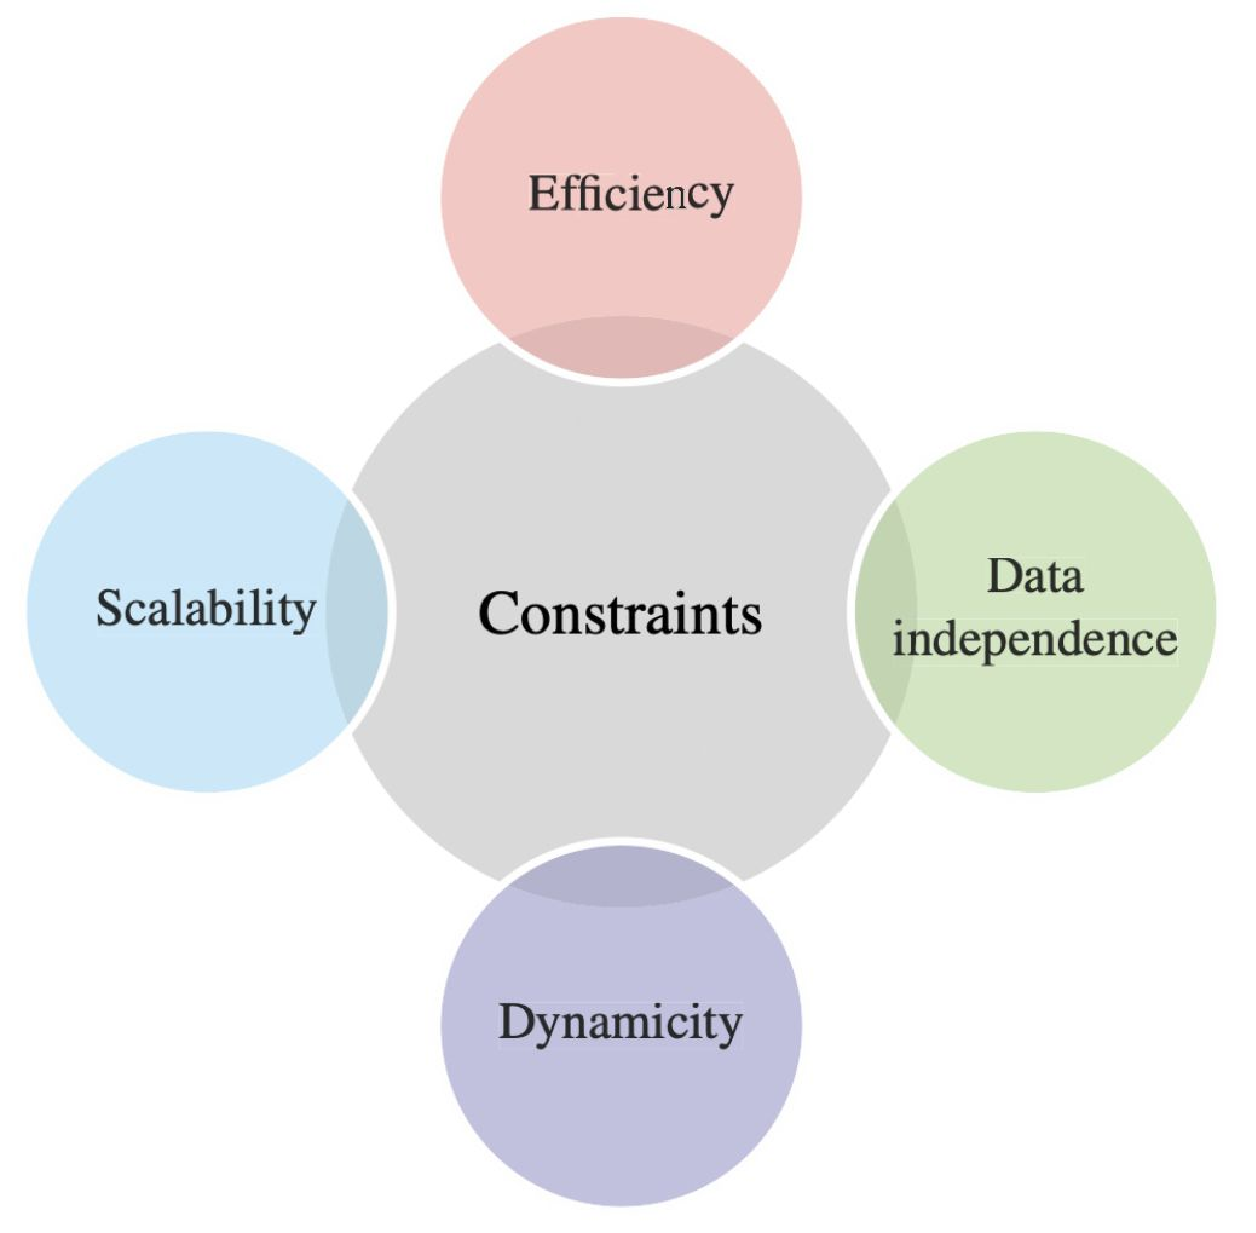
\includegraphics[width=0.6\textwidth]{poziadavky.pdf}
\caption{Požiadavky pri indexovani veľkých dát \cite{8807848}}
\label{f:poziadavky}
\end{figure*}

\subsection{Škálovateľnosť}
Výraz škálovateľnosť, rozšíriteľnosť, nám hovorí o schopnosti indexovacieho systému prispôsobiť sa postupne rýchlejšie narastajúcemu objemu dát. V bežnom svete to známená, že daný systém musí byť schopný spracovávať stále väčšie množstva nových dát bez výraznejšieho poklesu rýchlosti.\cite{8807848} Na to je potrebný optimalizovaný algoritmus a dátové štruktúry, aby bol tento systém schopný udržať výkon aj pri väčšom zvýšení záťaže. Obzvlášť v oblasti IoT kde sa prevažne pracuje s obrovským množstvom dát je táto vlastnosť nevyhnutná.

\subsection{Efektivita}
Efektivita (efektívnosť) spočíva v schopnosti systému poskytovať najrýchlejšiu možnú odozvu na dotazy vyhľadávania. \cite{Khettabi2022ClusteringAP} V jednoduchosti musí systém od odoslania požiadavky užívateľom v čo najkratšom čase doručiť relevantný výsledok. Ďalej efektivita zahŕňa aj výber vhodných algoritmov, pretože výpočet podobnosti objektov môže byť značne náročnejší.

\subsection{Dynamickosť}
Dynamickosť (dynamika) znamená schopnosť za čo najmenší čas reagovať na zmeny dátach a databáze bez nutnosti reorganizácie, ktorá by zabrala príliš veľa času. To nám umožňuje mať nepretržitú indexáciu a stále aktuálne údaje.\cite{8807848} V dnešnom svete Internetu vecí je tato špecifikácia z dôvodu nutnosti zmien a pridávania nových zariadení taktiež nevyhnutná.

\subsection{Nezávislosť na dátach}
Táto vlastnosť umožňuje indexovaciumu systému účinnosť aj v prípade, že sa na vstupe objavia rôzne typy dát ako aj ich rozloženie. Najmä v oblasti IoT kde sú mnoho krát rôzne formáty, štruktúry a značkovanie dát, musí byť schopný tieto údaje efektívne spracovať, bez ohľadu na ich charakteristiky.\cite{2021} To robí nezávislosť na dátach neoddeliteľnú súčasť Internetu vecí.


\section{Oblasti využitia} \label{oblasti}
Spektrum využitia Internetu veci je veľmi široké. Dôvody používania sú rôzne, či už je to kvôli zvýšeniu efektivity, zníženiu nákladov alebo celkovému zlepšeniu kvality produktov, či služieb. Aplikácia indexovania big IoT dát je široká a zohráva kľúčovú úlohu v mnohých odvetviach. 


\subsection{Využitie v zdravotníctve}
Aplikácia veľkých dát spojených s IoT v oblasti zdravotnej starostlivosti je novým a pomerne rýchlo sa rozvíjajúcim oblastným výskumom. Využitie zariadení a senzorov internetu vecí umožňuje zdravotnému personálu jednoducho zbierať a analyzovať veľké množstvo dát v reálnom čase, čo prispeje k lepším výsledkom pacientov, lepšej prevencií, zníženiu nákladov, či celkovému zlepšeniu kvality zdravotnej starostlivosti.\cite{2021}
Stále využívanie internetu vecí a veľkých dát v oblasti zdravotníctva má vysoký potenciál prispieť k udržateľnejšiemu rozvoju. Technológia IoT má významné uplatnenie najčastejšie v oblastiach zdravotnej starostlivosti, ako je monitorovanie UV žiarenia, zubná starostlivosť, či detekcia pádov.\cite{Singh2020EmergenceOI}
Napriek tomu v spojitosti s touto témou vzniká mnoho problémov a výziev, ktorým treba čeliť. Či už sú to problémy s ochranou osobných údajov, bezpečnosti a mnoho ďalších, ktoré budú všetky spomenuté v jednej z posledných kapitol (časť .~\ref{vyzvy}).



\subsection{Využitie v priemysle}
Veľké množstvo údajov má v priemyselnom odvetví mimoriadny význam, pretože slúži na zlepšenie a potenciálne urýchlenie výrobných procesov. Tieto rozsiahle zdroje údajov, často označované ako "priemyselné údaje IoT" (internet vecí), pochádzajú z rôznych snímačov, meracích prístrojov a automatizovaných systémov vo výrobných zariadeniach. Zahŕňajú informácie týkajúce sa veličín, ako sú teplota, tlak, vlhkosť, stav strojov, spotreba energie a množstvo ďalších parametrov. \cite{Zhou2021VariationalLE}


\subsection{Využitie vo výskume}
Výskumníci už aj v dnešnej dobe skúmaju potencionálne využívanie a dôsledky technológie internetu vecí pomocou veľkých objemov dát. Predpokladá sa \cite{Riggins2015ResearchDO}


\section{Techniky indexovania veľkých dát v IoT} \label{techniky}
Techniky použité pri indexovaní údajov musia byť čo najefektívnejšie, čo vôbec neuľahčuje príchod nových a objemnejších typov dát. Z dôvodu veľkého počtu techník indexovania objemných dát v internete vecí sú v tejto kapitole spomenuté iba tie najviac rozšírené.

\paragraph{}
\begin{figure*}[tbh]
    \centering
    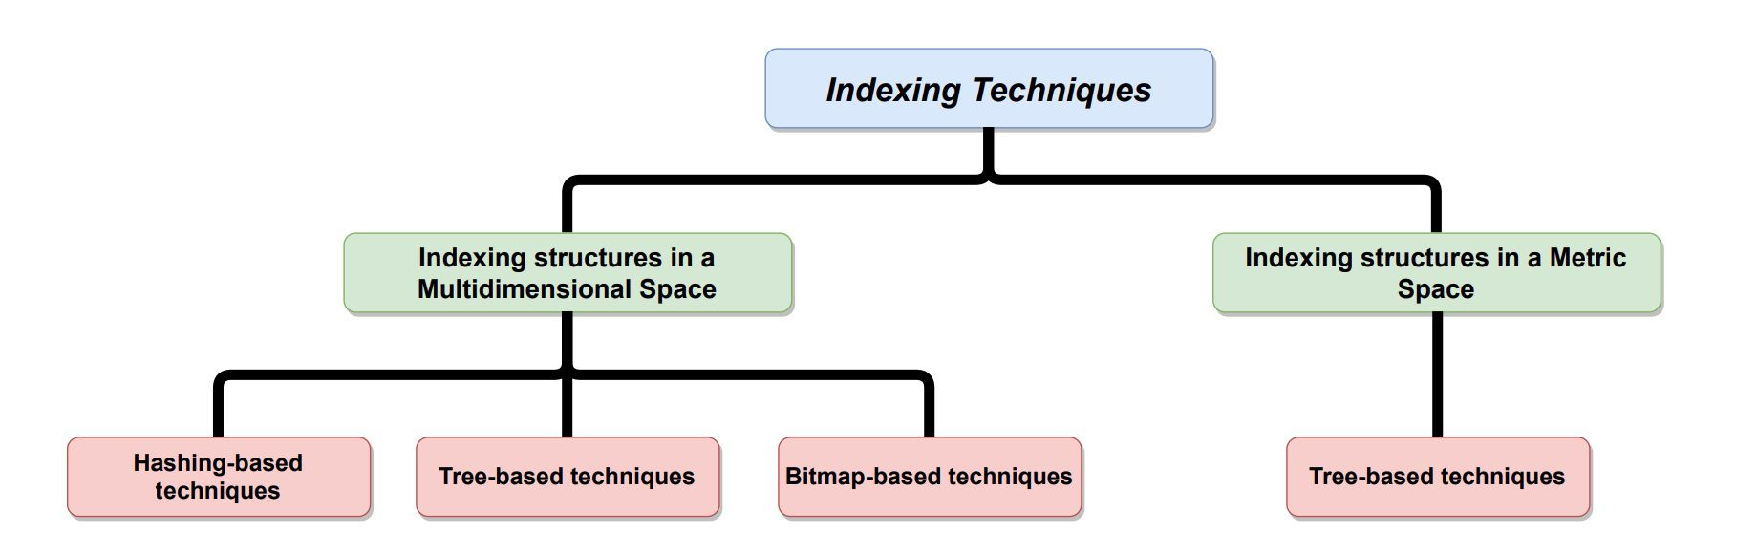
\includegraphics[width=1\textwidth]{techniky.pdf}
\caption{Globálna taxonómia techník indexovania \cite{2021}}
\label{f:techniky}
\end{figure*}

\subsection{Techniky založené na stromoch (Tree-Based)}
 Technika Tree-Based sa používa na indexovanie viacrozmerných údajov na základe rozdielenia priestoru na podpriestory alebo bunky.\cite{2021}


\subsubsection{R*Q-tree}
\subsubsection{BB-tree}
\subsubsection{Kd-tree}
\subsubsection{Quad-tree}
\subsubsection{Pyramid-tree}

\section{Výzvy} \label{vyzvy}




\section{Záver a zhrnutie} \label{zaver}

\section{Reakcia na témy z prednášok} \label{temy}

\newpage
\bibliography{literatura}
\bibliographystyle{unsrt}
\end{document}
